\cleardoublepage
\section{外文翻译}
\renewcommand{\theequation}{\arabic{equation}}
\renewcommand{\thefigure}{\arabic{figure}}
\begin{center}
    \zihao{3}\textbf{文献翻译标题}
\end{center}
\begin{center}
	\zihao{4}S. H. It, O. M. Gaster\\
	\zihao{5}（摘自：Noture 321, 1145 (2048)）
\end{center}
\subsection*{摘要}

\settocdepth{part} % 以下部分不计入目录

% 注：正文部分的subsection中公式和图表的编号会在每一个subsection中重新开始计数，如果需要在整个文档中保持编号的连续性，可以在每个subsection后加上以下两行代码：
% \setcounter{equation}{上一个subsection中最后一个公式的编号}
% \setcounter{figure}{上一个subsection中最后一个图表的编号}
\subsection{引言}

\subsection{章节1.2}
插入一个图片
\begin{figure}
    \centering
	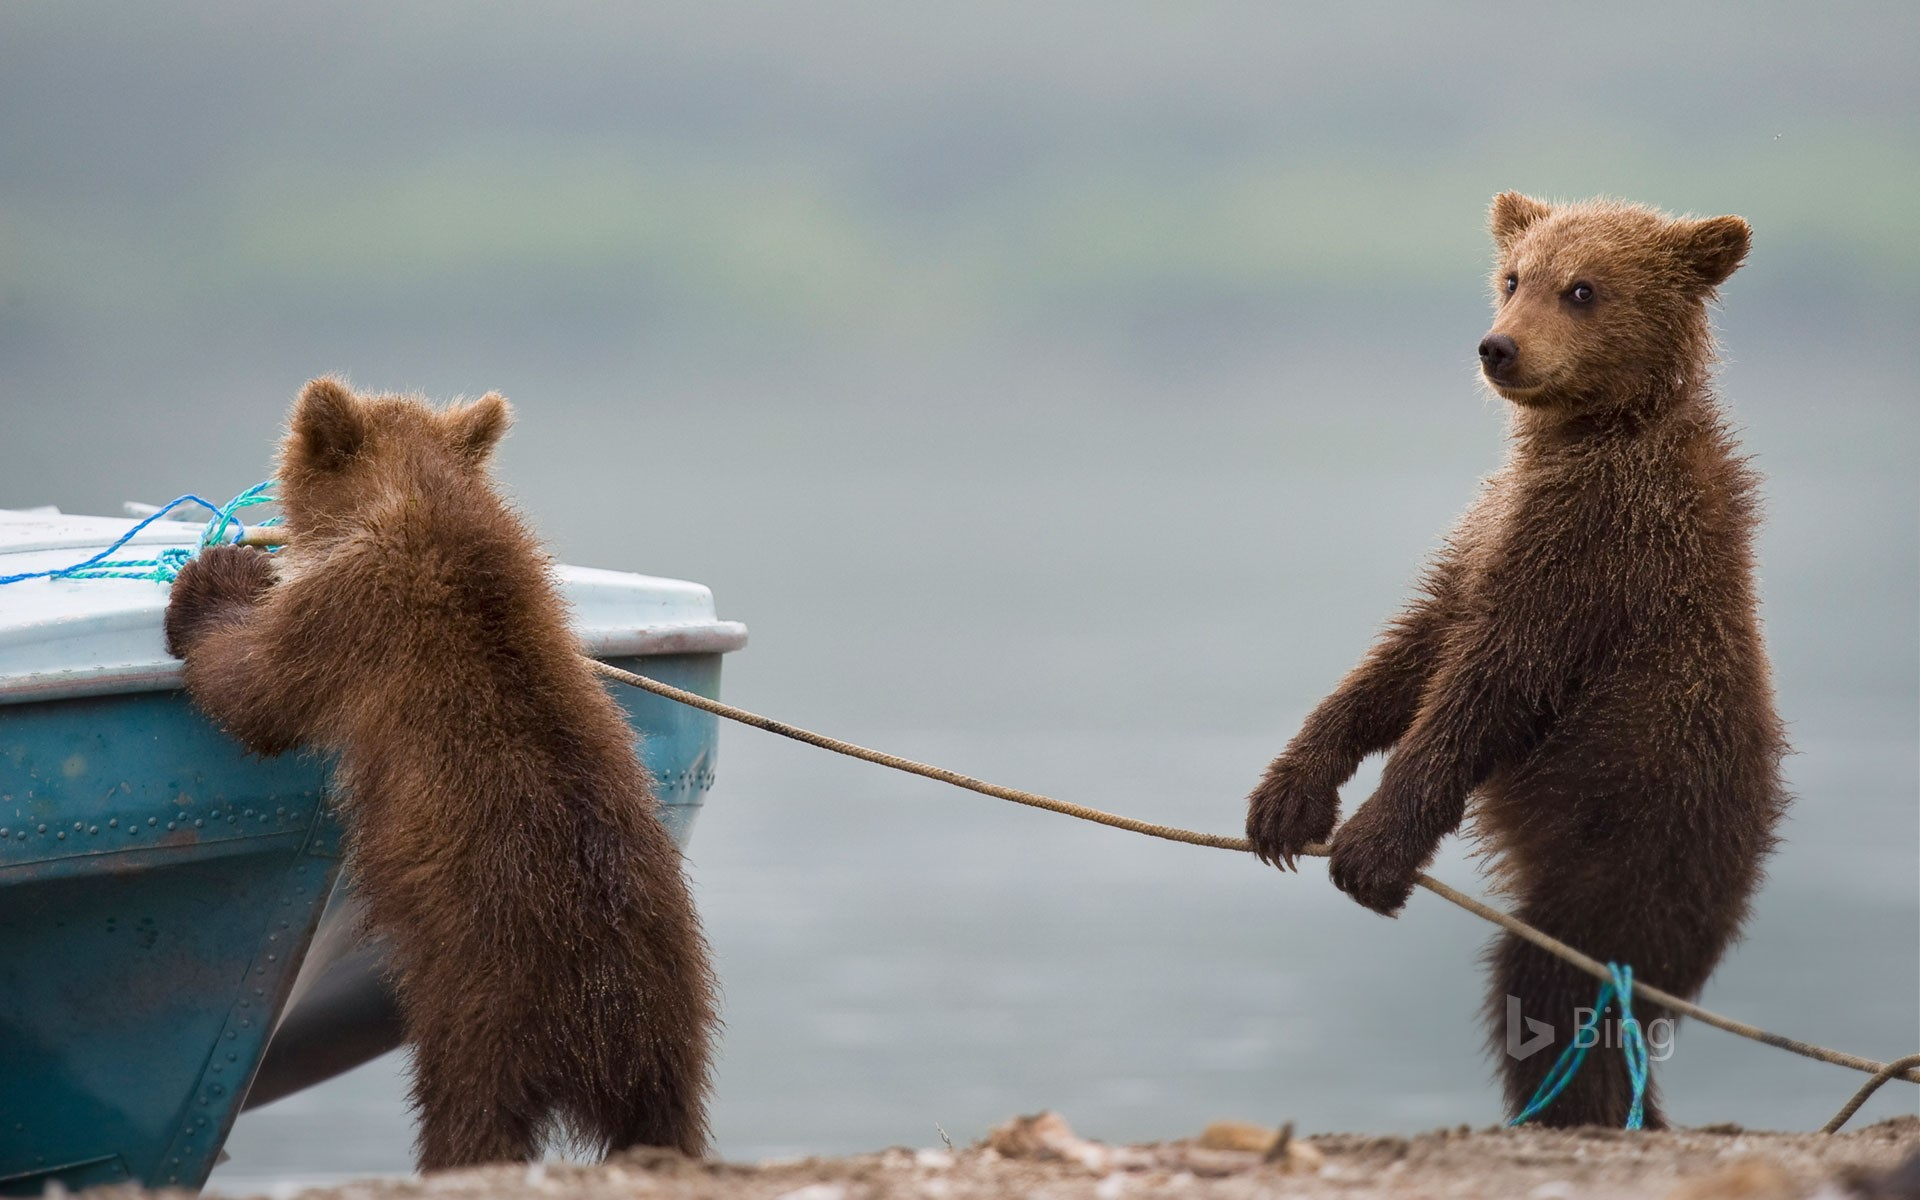
\includegraphics[width=0.5\textwidth]{images/BingWallpaper-2019-04-01.jpg}
	\caption{figure one}
	\label{fig:figlabelone}
\end{figure}
引用图片1 \ref{fig:figlabelone}

多空一行表示分段

这是一个公式
\begin{equation}
	\label{eq:one}
E = mc^2
\end{equation}
引用公式 \eqref{eq:one}
\subsection{章节1.3}
\setcounter{figure}{2}


\begin{figure}
    \centering
	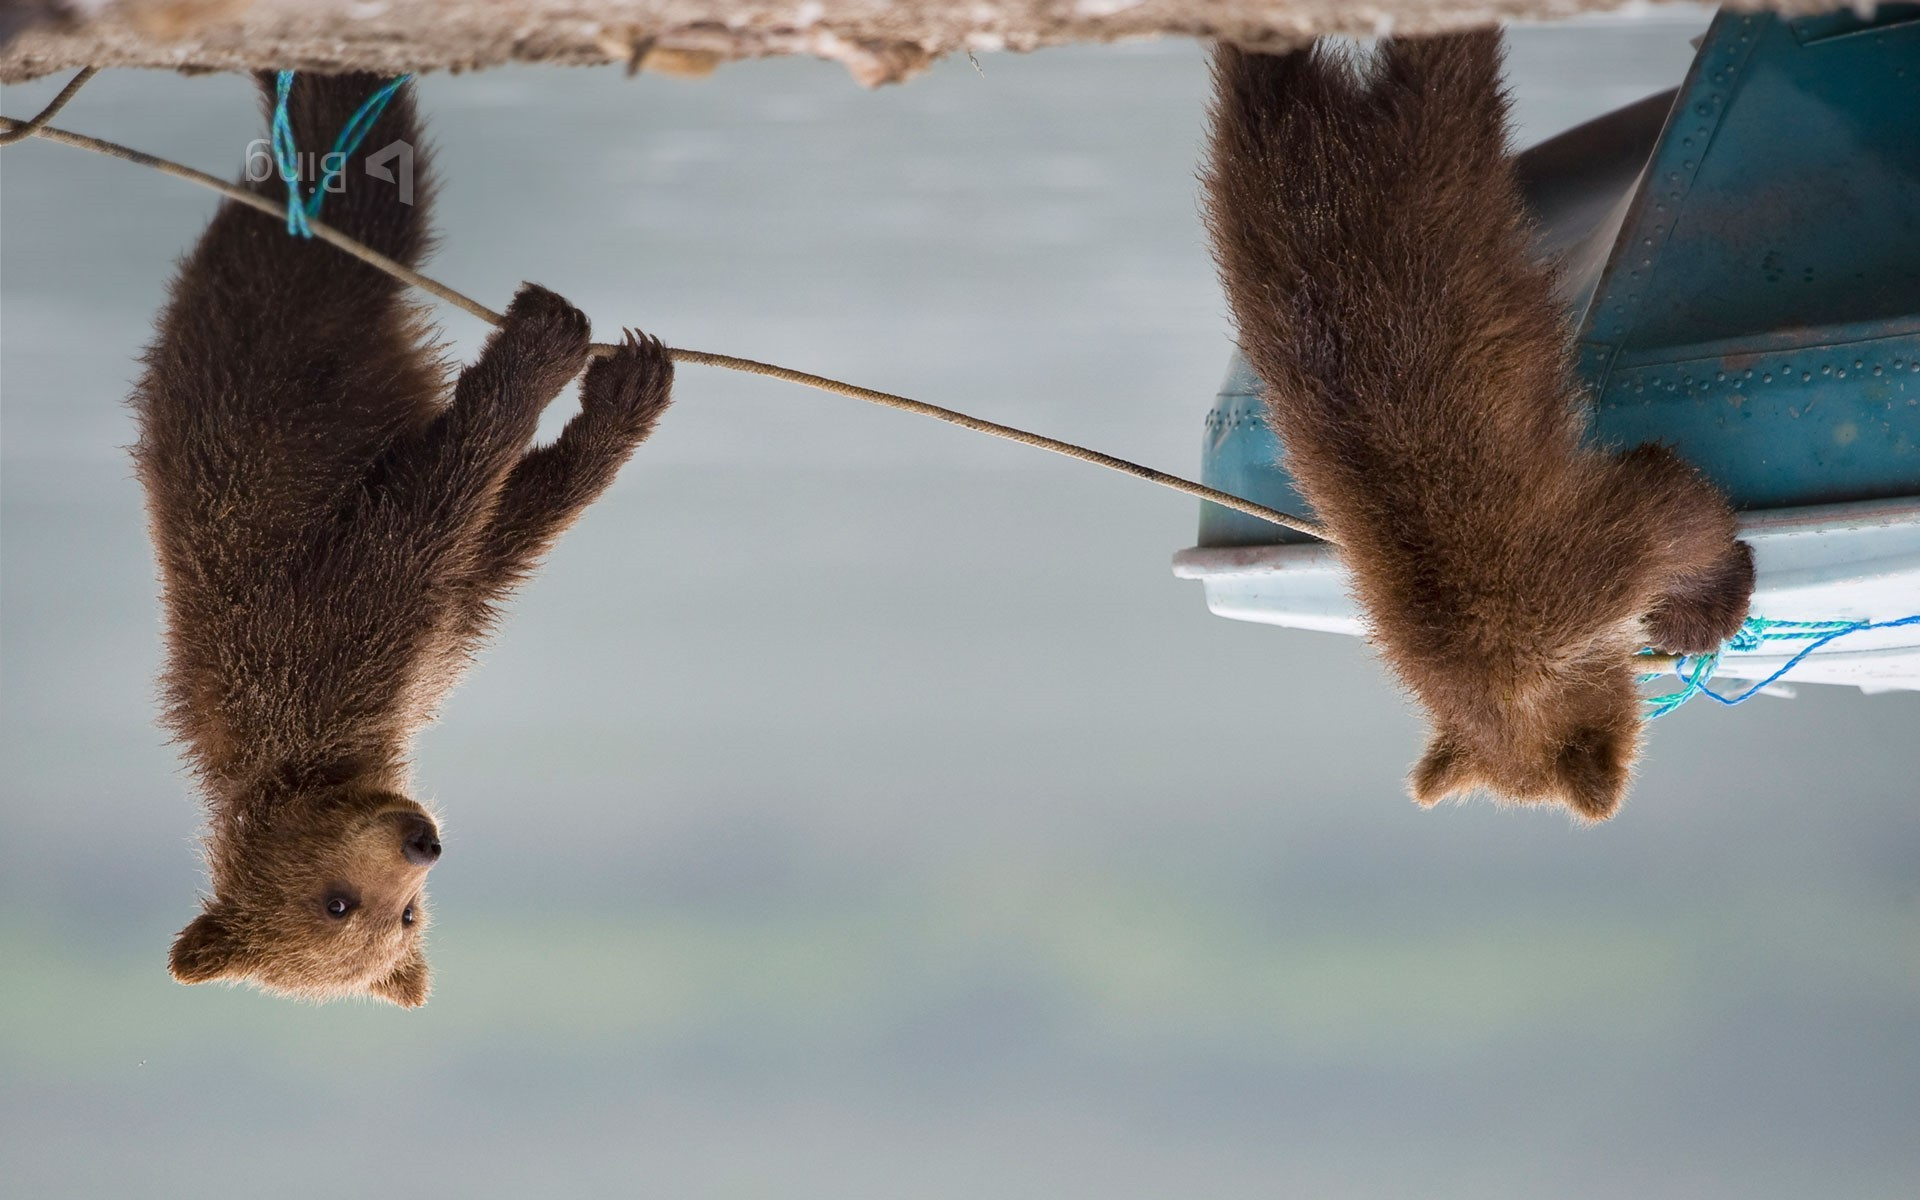
\includegraphics[width=0.5\textwidth]{images/BingWallpaper-2019-04-01 - 副本.jpg}
	\caption{figure two}
	\label{fig:figlabeltwo}
\end{figure}
引用图片2 \ref{fig:figlabeltwo}

引用文献1 \upcite{article1} 文献2\upcite{article2}
引用多篇文献 \upcite{article1,article2}

\subsection{结论}

% 参考文献
\clearpage
\bibliographystyle{gbt7714-numerical}
\phantomsection		% 要想目录中参考文献的超链接正确需要加这一语句
\subsection{参考文献}
{\normalfont\CJKfamily{Songti}\zihao{5}\setlength{\baselineskip}{14pt}
\renewcommand{\refname}{\vspace{-\baselineskip}}
\bibliography{reference/translations}}

\resettocdepth % 恢复目录计数